\section{Task 3 --- Generating a Certificate for your server}
%
\begin{lstlisting}[language=bash, caption=A command generating the
    certificate for the server]
    openssl ca -config demoCA_openssl.cnf \
        -policy policy_anything -md sha256 -days 3650 \
        -in server.csr -out server.crt -batch -cert ca.crt \
        -keyfile ca.key
\end{lstlisting}

\begin{figure}
    \centering
    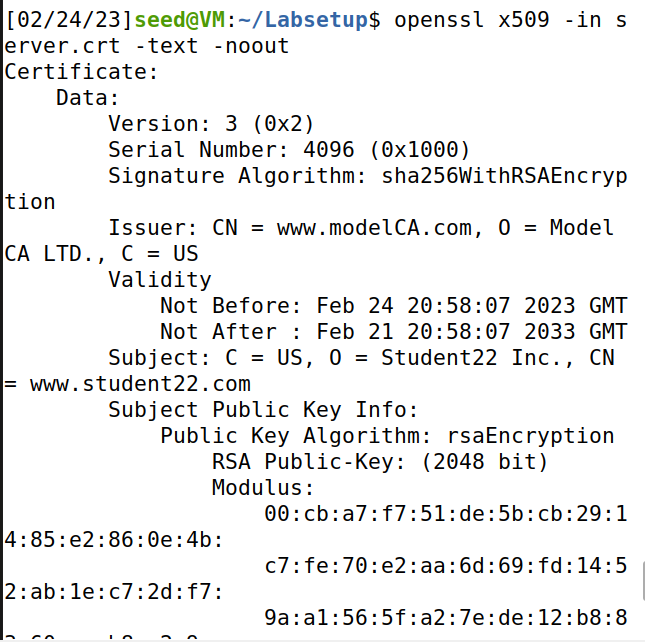
\includegraphics[height=\textheight,width=\textwidth,keepaspectratio]
    {figures/server_crt.png}
    \caption{Decoded certificate of the server {\fontfamily{qcr}\selectfont
    www.student22.com}.}\label{fig:server_crt}
\end{figure}

\begin{figure}
    \centering
    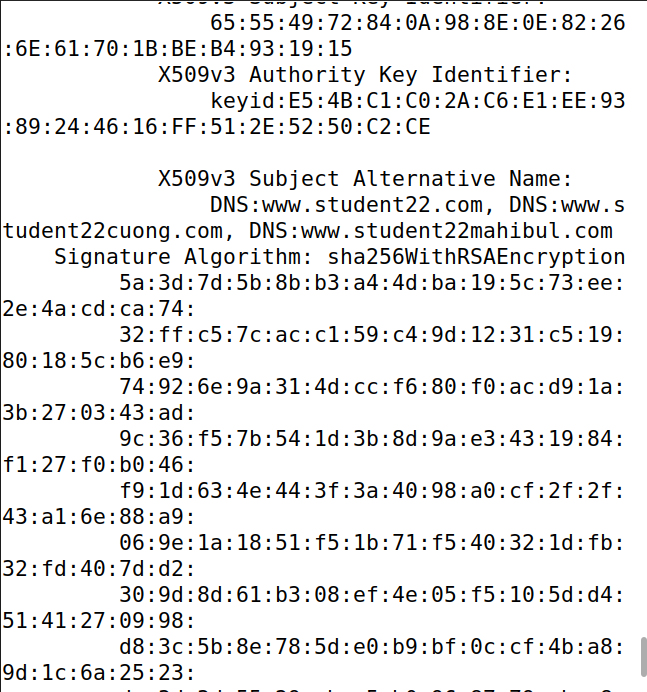
\includegraphics[height=\textheight,width=\textwidth,keepaspectratio]
    {figures/extension_server_crt.png}
    \caption{Alternatives names are included.}\label{fig:alter_name_incl}
\end{figure}

\autoref{fig:server_crt} shows partly the certificate of {\fontfamily{qcr}\selectfont
www.student22.com}. \autoref{fig:alter_name_incl} illustrates that alternative
names which are embedded in {\fontfamily{qcr}\selectfont openssl ca} are
included in the output certificate.